\chapter{基于局部的特征提取算法}
\label{cha:local}
在上一节的学习过程中,笔者渐渐感觉到计算算子对人脸识别,分类系统的影响非常大,毕竟,人脸图像被分解后,仅仅由一个很短的向量来表示,那该编码系统对样本的区分程度很大程度上就能决定后续分类系统的性能.因此,我渐渐发现了基于局部的特征提取算法,它们有些具有\textit{Content Awareness}的特性,对背景噪声有一定的区分能力,并且可以精细的比较样本的细节之处,因此可以达到精确的识别性能.本章节以SIFT算子为例做介绍.

\section{SIFT}
\subsection{SIFT的原理}
本章节主要基于\cite{lowe2004distinctive, issolah2013sift, juan2009comparison, siftopencv, siftvlfeat, siftubc,lowe1999object},在Matlab中使用了\cite{siftvlfeat}实现的SIFT算法. \newline

SIFT算子的计算方法共分4步.
\begin{enumerate}
	\item SIFT首先构建一系列DoG(Difference-of-Gaussian)金字塔.并在其上计算极值,作为该层空间上的特征点.具体的计算方法是求得所有满足在其$3 \times 3$临域上为最大值或最小值的点. 

	 	\begin{center}
		\begin{minipage}[t]{\linewidth}
		%\label{fig:main}
		\center
		{
		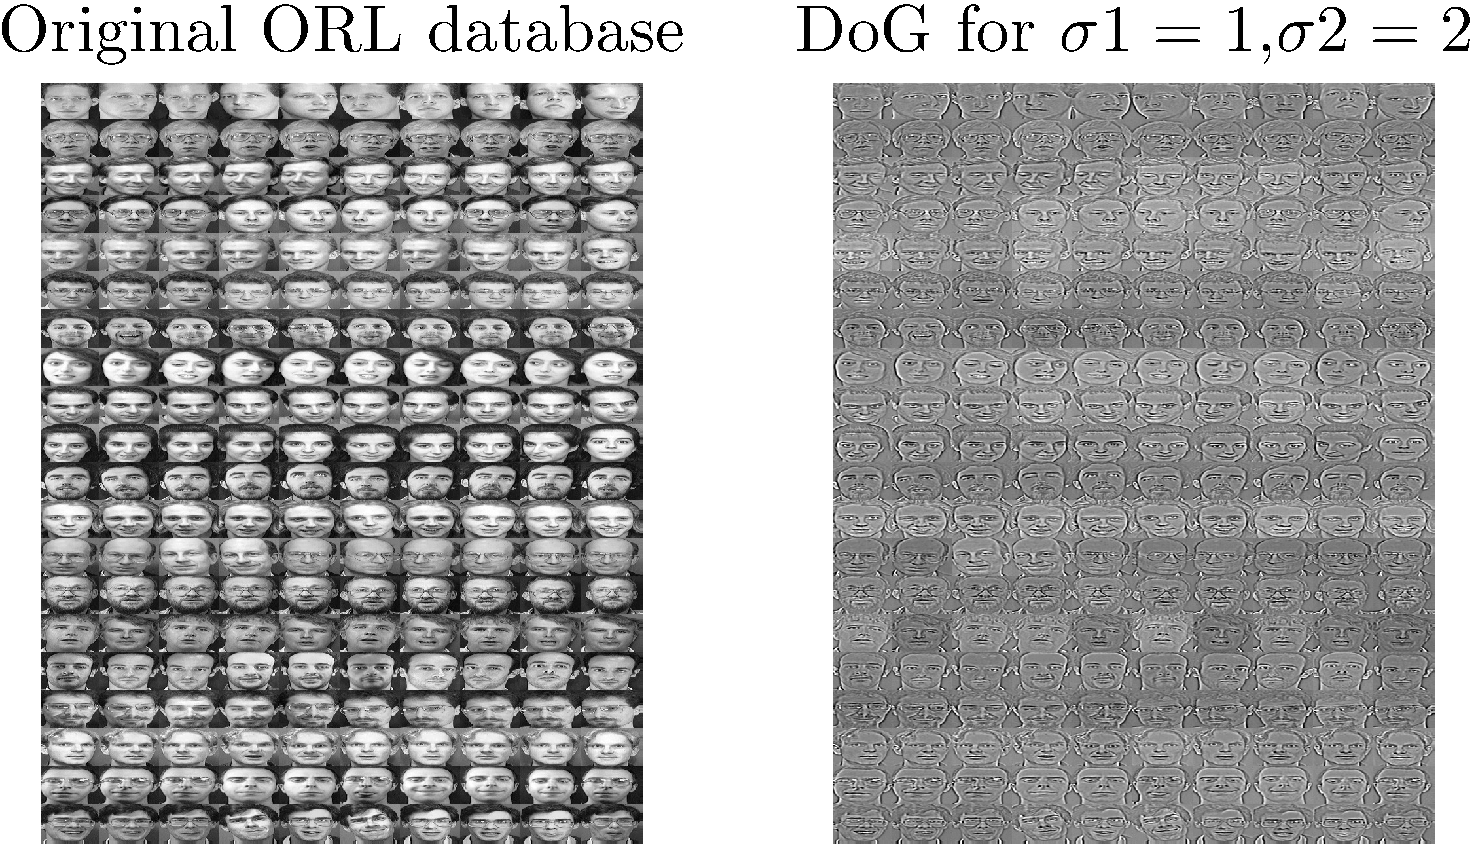
\includegraphics[width=\textwidth]{Img/c3/dog_demo} \captionof{figure}{DoG滤波示意图,DoG图像采用了和输入图像相同的尺度}
		}
		\end{minipage}
		\medskip
		\end{center}
	
	\item 当每层的特征点被计算出来后, SIFT计算该层求得的特征点是否在解析度更大的一层上也满足为最大值或最小值.只有一直满足该特性的点才能被下一步运算.运算结束后,SIFT再一步过滤掉因噪音,边界而被误判为特征点的点.SIFT空间保留了差值运算中特征点相对最初一层邻域的尺度,以及特征点的位置作为特征点的描述.
	\item SIFT在计算出特征位置上每隔$10^\circ$的梯度,并选择梯度最大及三个以内的大于某阈值梯度的方向为该特征位置的方向.经过以上三步,SIFT计算出了输入图片的特征点.
	
		 \begin{center}
		\begin{minipage}[t]{\linewidth}
		%\label{fig:main}
		\center
		{
		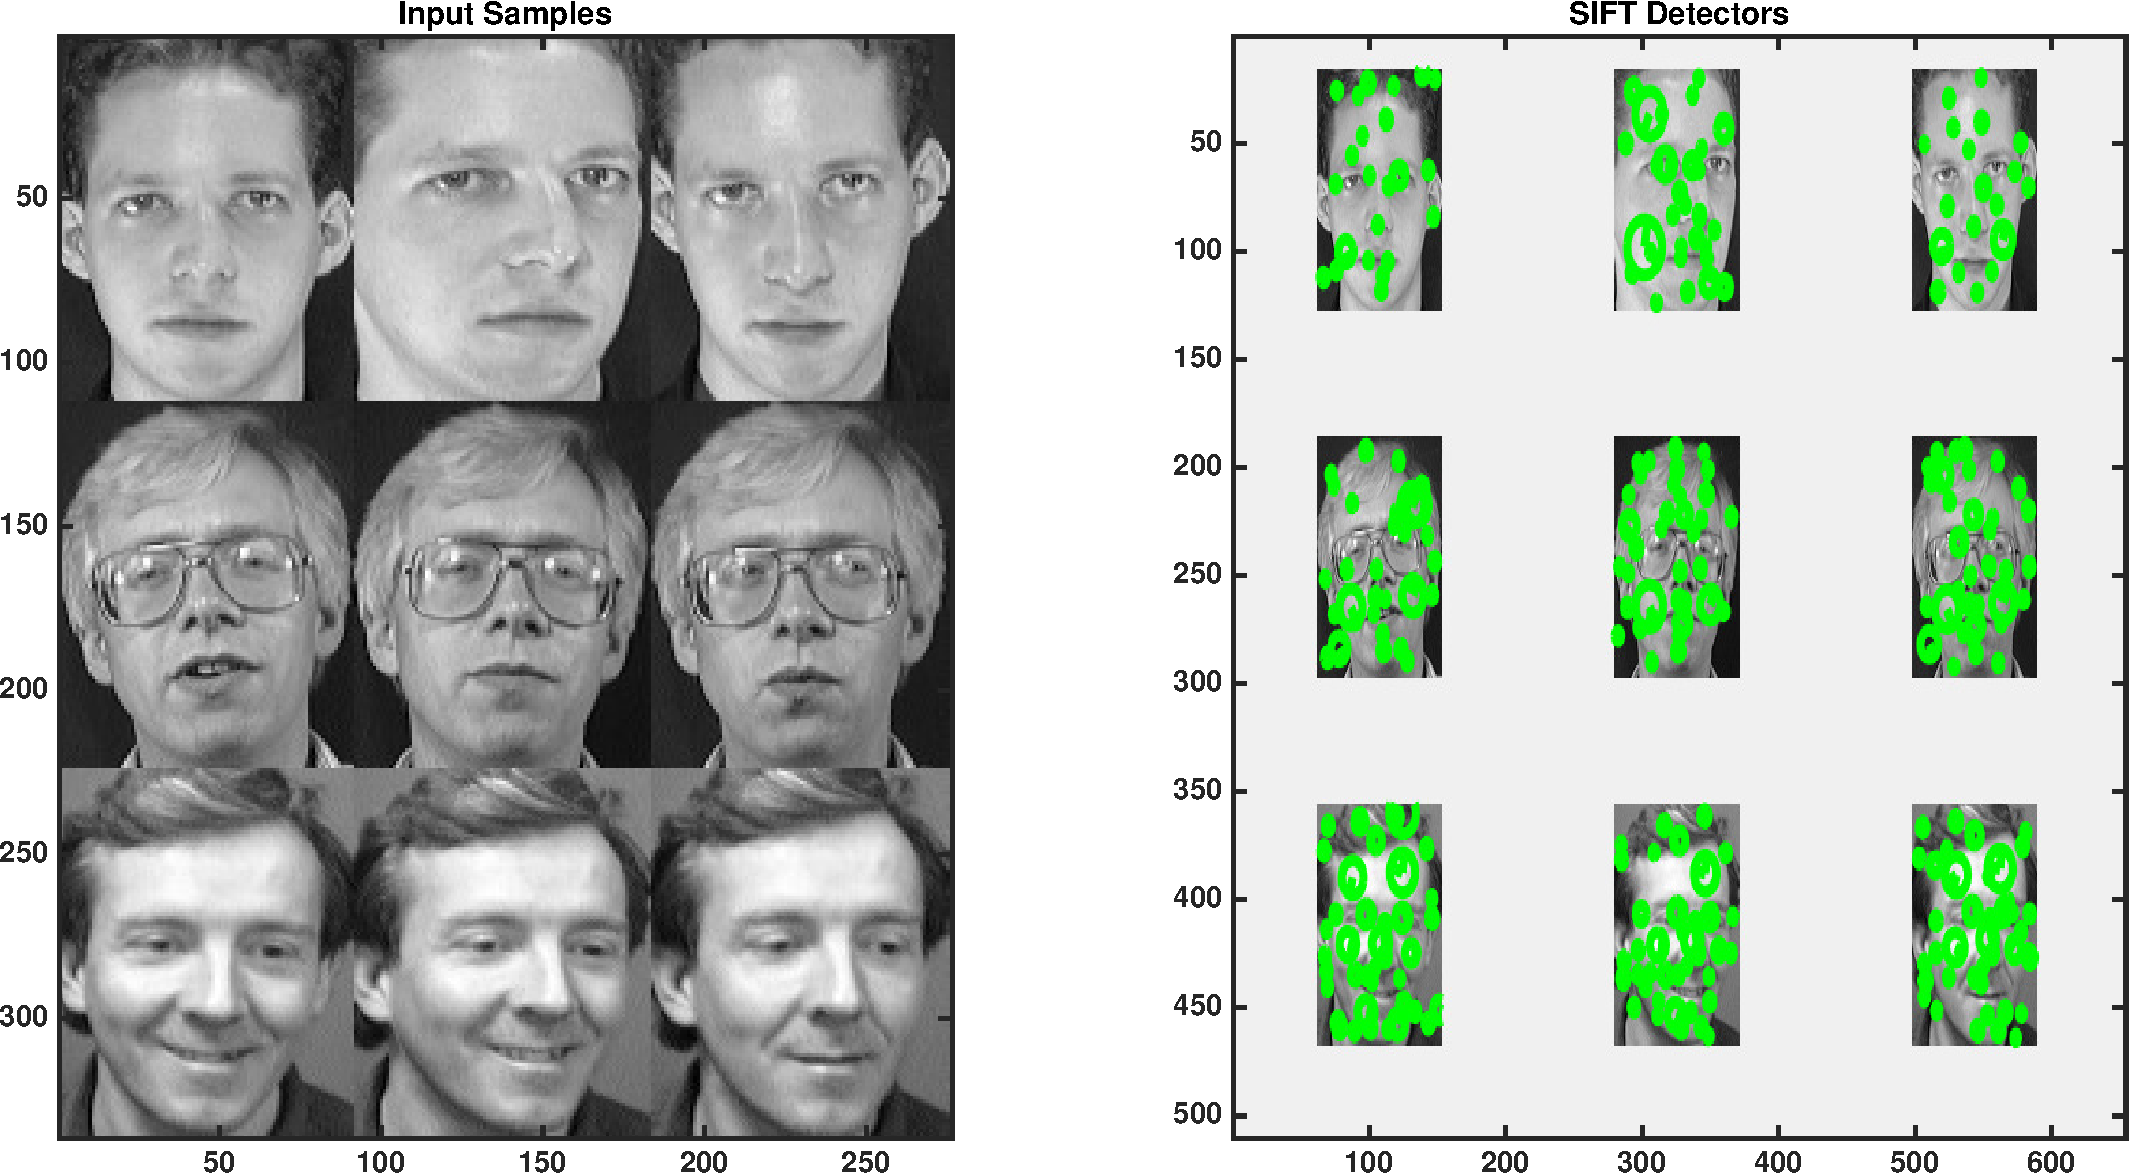
\includegraphics[width=\textwidth]{Img/c3/sift_detectors.pdf} \captionof{figure}{SIFT特征点示意}
		}
		\end{minipage}
		\medskip
		\end{center}
	\item 最后一步是对特征点的描述,SIFT采用一个$N_\theta \times N_x \times N_y$(通常为$8 \times 4 \times 4$,其中$\theta$,$x$,$y$取不同的值,并分别在特征空间上计算梯度)的向量(又称HoG, Histogram of Gradients)来描述该特征点的性质.在\textit{SIFT-PCA}算法采用了另一种方法.
		\begin{center}
		\begin{minipage}[t]{\linewidth}
		%\label{fig:main}
		\center
		{
		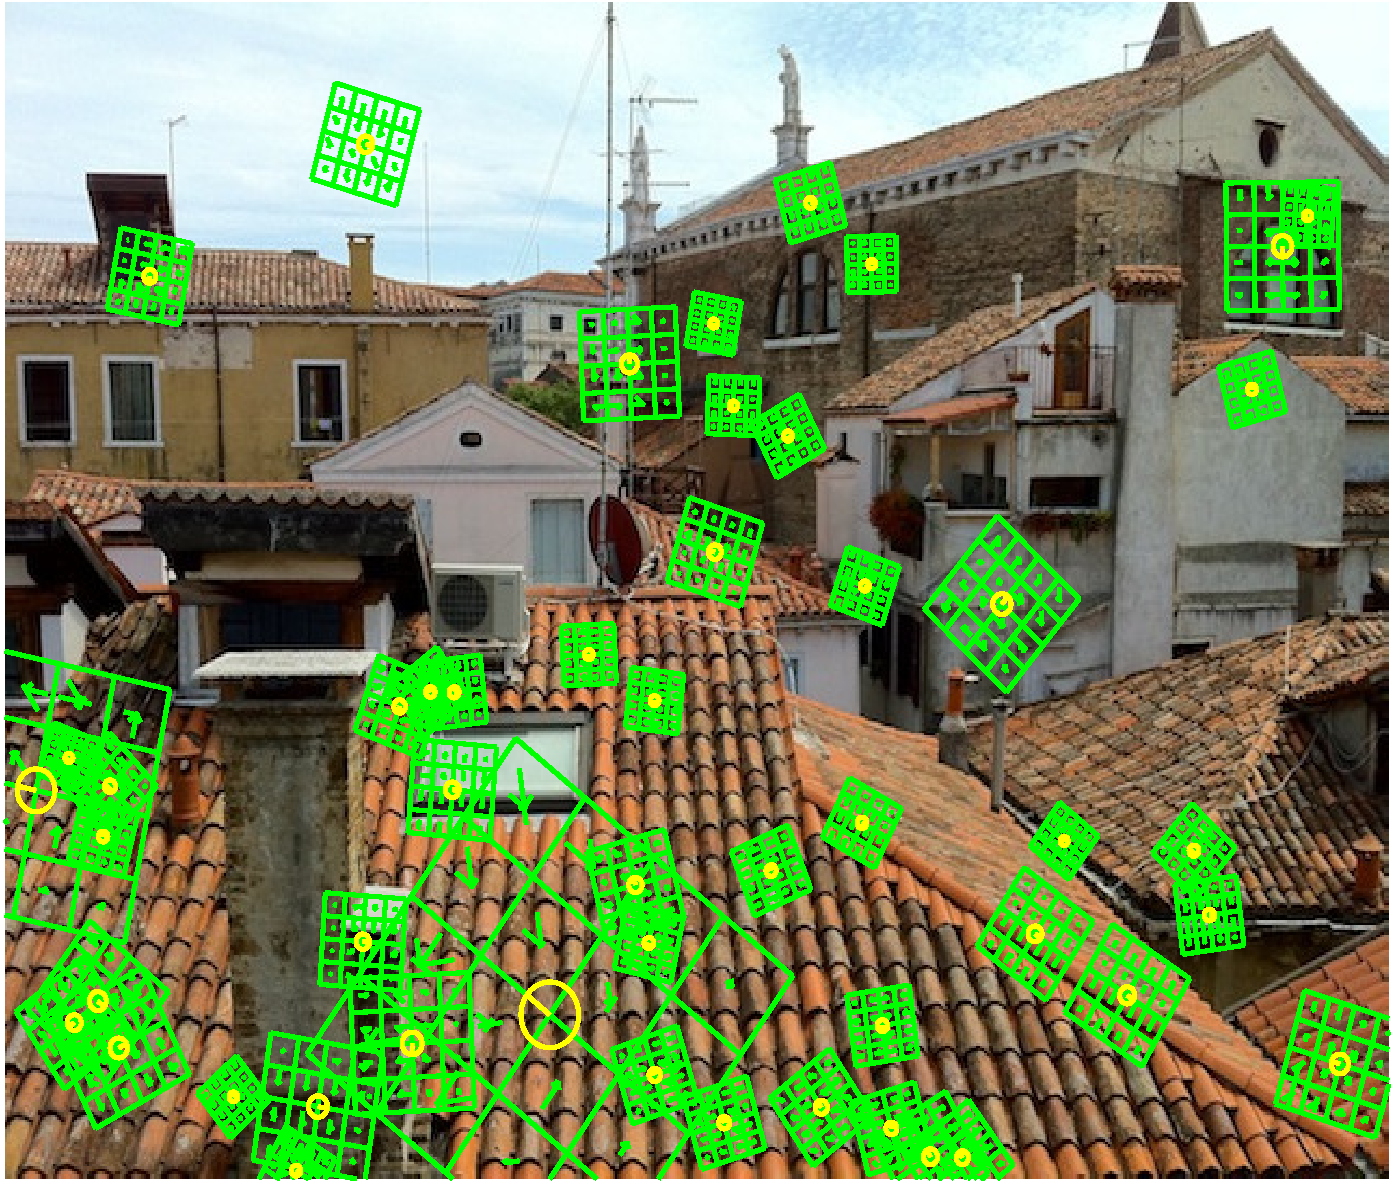
\includegraphics[width=\MyFactor\textwidth]{Img/c3/sift_demo} \captionof{figure}{SIFT特征点的描述,来源\cite{siftvlfeat}}
		}
		\end{minipage}
		\medskip
		\end{center}
		上图就是通常的SIFT描述的表示方法,可见,它是由一个$4 \times 4$的方阵表示的,分别表示了特征点所确定的特征空间的x,y取值的梯度.而每个方阵内部又由一个8个方向变化长度的向量表示,向量的长度表示了在该方阵x,y确定的位置上,不同$\theta$下的梯度大小.总计共有128($8 \times 4 \times 4$)个向量来描述特征点所对应的特征空间.
	\end{enumerate}



\subsection{SIFT-PCA算法}
由于SIFT运算结果过长,笔者实现了SIFT-PCA算子\cite{ke2004pca},它是一种采用块压缩技术的基于SIFT的1-3步的方法.具有可调节的长度.

	 	\begin{center}
		\begin{minipage}[t]{\linewidth}
		\center
		{
		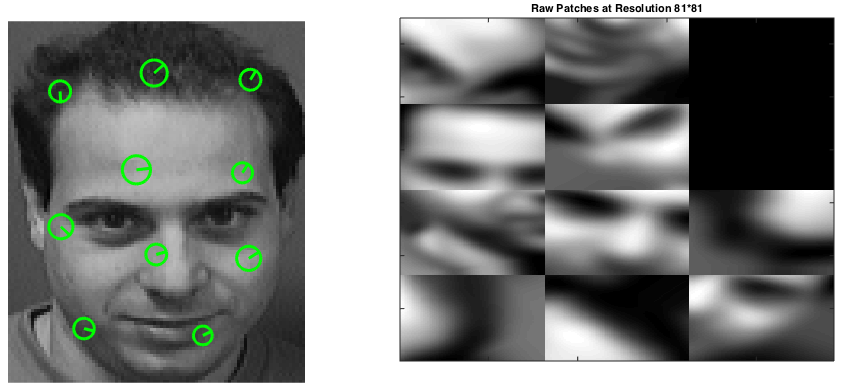
\includegraphics[width=\MyFactor\textwidth]{Img/c3/sift_raw_patch2} 
		\captionsetup{justification=centering}
		\captionof{figure}{SIFT特征点和对应的特征空间示意\\ 为了演示方便,图像中特征点对应$81 \times 81$的邻域,而实际计算中特征点对应$41 \times 41$的邻域}
				\label{fig:sift_patches}
		}
		\end{minipage}
		\medskip
		\end{center}
	
	它的具体步骤是建立在SIFT算法的1到3步上的,在标准特征位置所描述的空间上:
	\begin{enumerate}
		\item SIFT-PCA算法首先计算该空间的水平,竖直两个梯度空间(本文中使用了Sobel方法).同时,为了避免边界梯度的骤增,边界的梯度被剔除了.
			
		\begin{center}
		\begin{minipage}[t]{\linewidth}
		\center
		{
		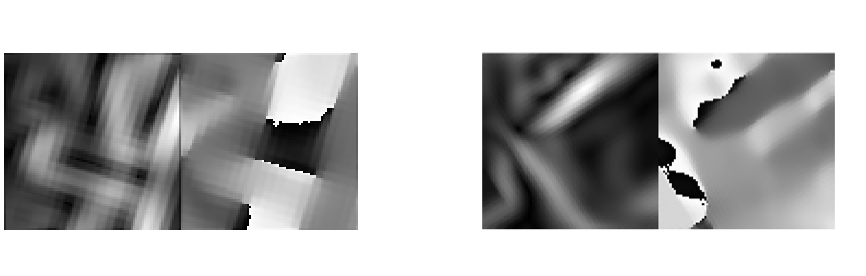
\includegraphics[width=\MyFactor\textwidth]{Img/c3/gradient.png} 
		\captionsetup{justification=centering}
		\captionof{figure}{水平,竖直两个梯度空间示意\\ 左:使用Sobel算子,右:使用prewitt算子\\ 计算\ref{fig:sift_patches}第一张图片的特征空间}
		}
		\end{minipage}
		\medskip
		\end{center}
		
		\item SIFT-PCA计算多张图片多个特征点上的梯度空间,并且使用PCA对其进行降维运算
		\item 当新输入空间时,SIFT-PCA使用标准SIFT算法提取特征点及特征点对应的空间,计算出对应空间的水平,竖直梯度空间后,对这两个空间使用上一步的基底降维.坐标就是SIFT-PCA对特征点对应的描述
	\end{enumerate}
	本文实现中,使用了100个人所提取出的特征梯度空间用作SIFT-PCA基底的学习,并在3600左右的特征向量中取前20个作为PCA降维后的特征向量,降维后的前20特征值占据了约60\%的特征值,下面是PCA的特征值绘制:
	
			\begin{center}
		\begin{minipage}[t]{\linewidth}
		%\label{fig:main}
		\center
		{
		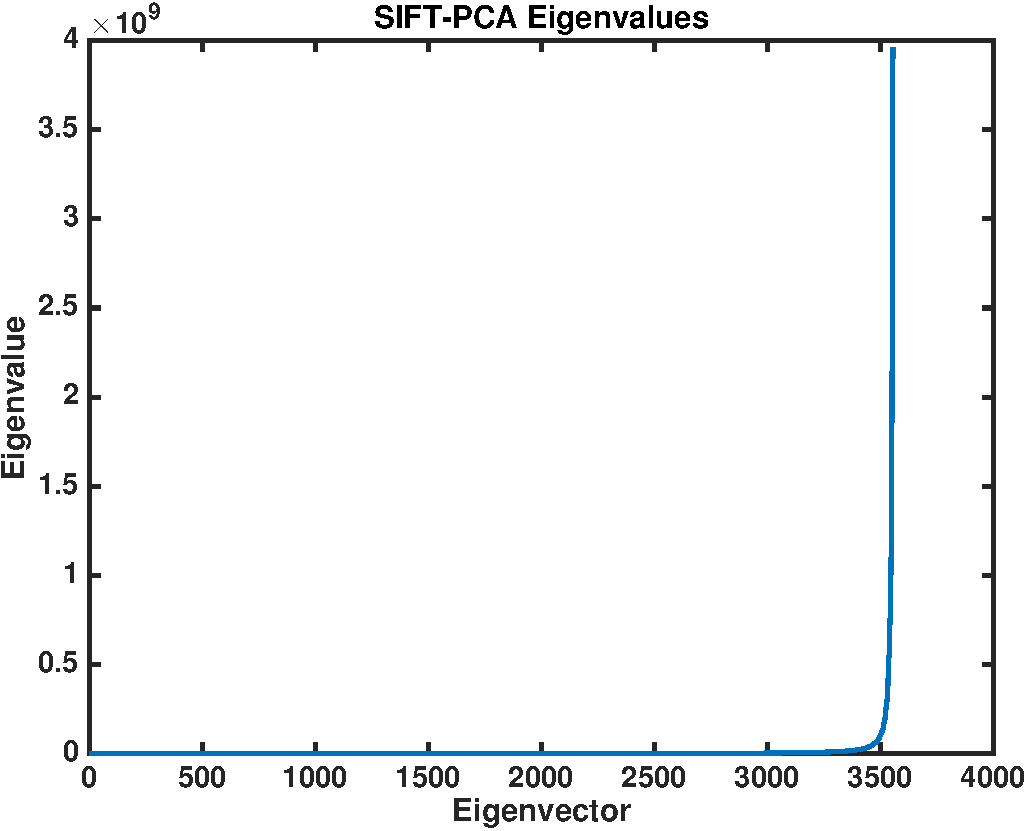
\includegraphics[width=\MyFactor\textwidth]{Img/c3/sift_pca_eigen} 
		\captionof{figure}{PCA的特征值}
		}
		\end{minipage}
		\medskip
		\end{center}
		
	经过SIFT-PCA后,SIFT算法原长度为128位的HoG特征描述就被PCA压缩为20位了.
		

\subsection{SIFT的编码方法}
由于SIFT算子是\textit{Content Aware}的,其特征提取的结果是由若干个特征点确定的特征空间来描述的.由于特征点的数目不确定,所以特征向量的总长度并不固定.这对后续的分类算法并不友好.因此,SIFT的结果大都被编码了,编码方法通常有以下的方法.\cite{chatfield2011devil}
	\paragraph{BoF: Bag-of-Features}
	BoW(Bag-of-Word)是文本处理中的手段,是指文本处理中,对文本的词汇分布作直方图的手段.也就是将该文本内所有出现过的词汇统计出来,并计算它们的出现频率.\newline
	
	BoF或BoVF(Bag-of-Visual-Features)是该BoW在局部特征提取的延伸手段,它统计了局部特征的特征点,当输入新样本时,样本在这些特征点的分布图就是它的全局特征.具体说来,BoF共分两步: \newline
	
	第一步是在输入样本之前,求得特征点分布重心的过程,它并不需要在输入样本时计算,可以离线提前求出.它的具体过程可以是:
	\begin{enumerate}
		\item 准备一些样本图像,并求得它们SIFT特征空间描述的全集
		\item 在这个全集上执行\textit{kmeans}运算,k值取值就是重心的数量,也就是之后全局样本的维度.并记录下重心的取值(也被成为\textit{Visual Vocabulary}).
	\end{enumerate}
	第二步是求得输入样本坐标的过程,它的过程可以是:
	\begin{enumerate}
		\item 取得样本的SIFT特征空间描述
		\item 对于每个描述,求得它最近重心,并被归到那一类里去
		\item 归类后,可以得到各个重心被归类的描述数目,而他们的分布就是该图像的BoF
	\end{enumerate}
	
	下面是结合标准的SIFT算法,分别取聚类个数为40,100,300,1500,3000的距离矩阵,计算BoW的样本有120张,总共提取了约4500个特征点,
	
		\begin{center}
		\begin{minipage}[t]{\linewidth}
		%\label{fig:main}
		\center
		{
		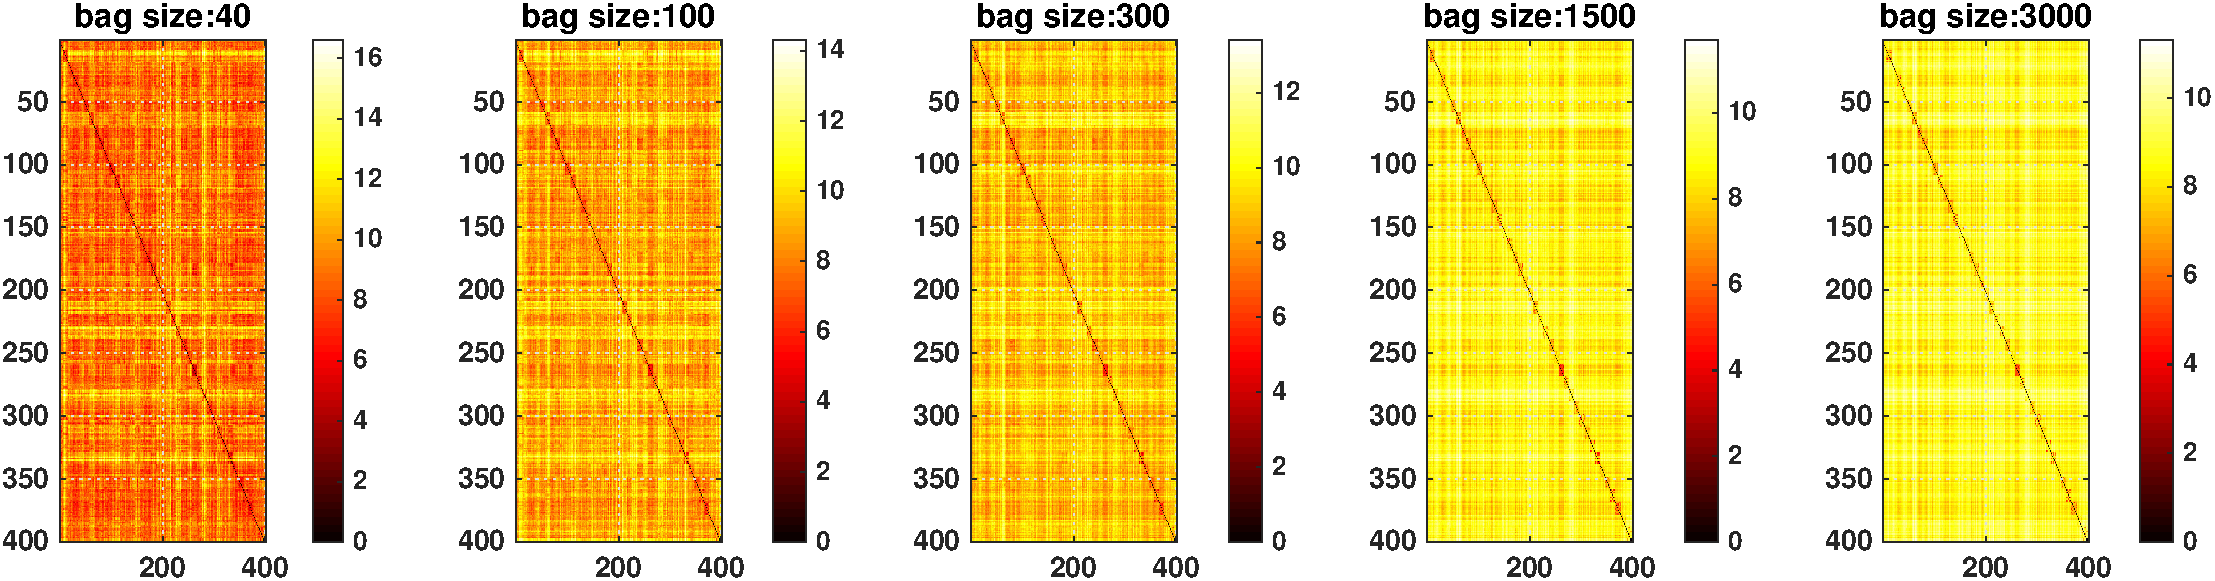
\includegraphics[width=\textwidth]{Img/c3/sift_bow_iter} 
		\captionof{figure}{BoW距离矩阵}
		}
		\end{minipage}
		\medskip
		\end{center}
		
		由此可见,BoW对人脸图像的泛化能力并不好,具体表现为类间距离和类内距离差别不大.而BoW的主要应用场所在于场景识别,对于人脸识别,由于人脸大都大同小异,所以聚类梯度的方法就不是很适用.
	\paragraph{在固定点计算描述}
	由于人脸图像的分布大体一致,该过程没有对特征的描述来分类,而是对特征的位置进行了分类,并且在固定的位置上计算它的描述.它的过程也分为两步,分别是离线的计算特征的位置,和在线的在固定的位置上计算特征的描述\newline
	
	第一步是离线计算特征点的位置,
	\begin{enumerate}
		\item 首先准备一些样本图像,并求得它们特征空间位置的全集
		\item 在这个四维空间(位置,尺度还有角度)的全集上执行\textit{kmeans}运算,k值得取值就是特征点的个数
	\end{enumerate}
	
				\begin{center}
		\begin{minipage}[t]{\linewidth}
		%\label{fig:main}
		\center
		{
		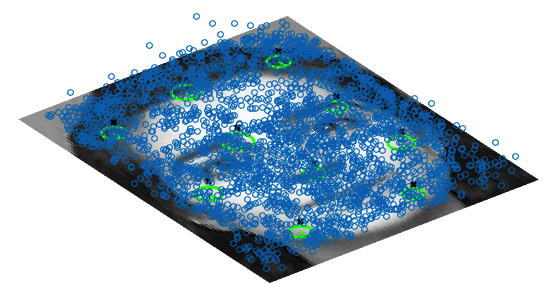
\includegraphics[width=\MyFactor\textwidth]{Img/c3/sift_face_kmeans} 
		\captionof{figure}{Kmeans计算过程示意\\ x,y:表征位置, z表征尺度,真实计算中,还涉及了角度}
		}
		\end{minipage}
		\medskip
		\end{center}
		下面是计算结果:
			\begin{center}
		\begin{minipage}[t]{\linewidth}
		%\label{fig:main}
		\center
		{
		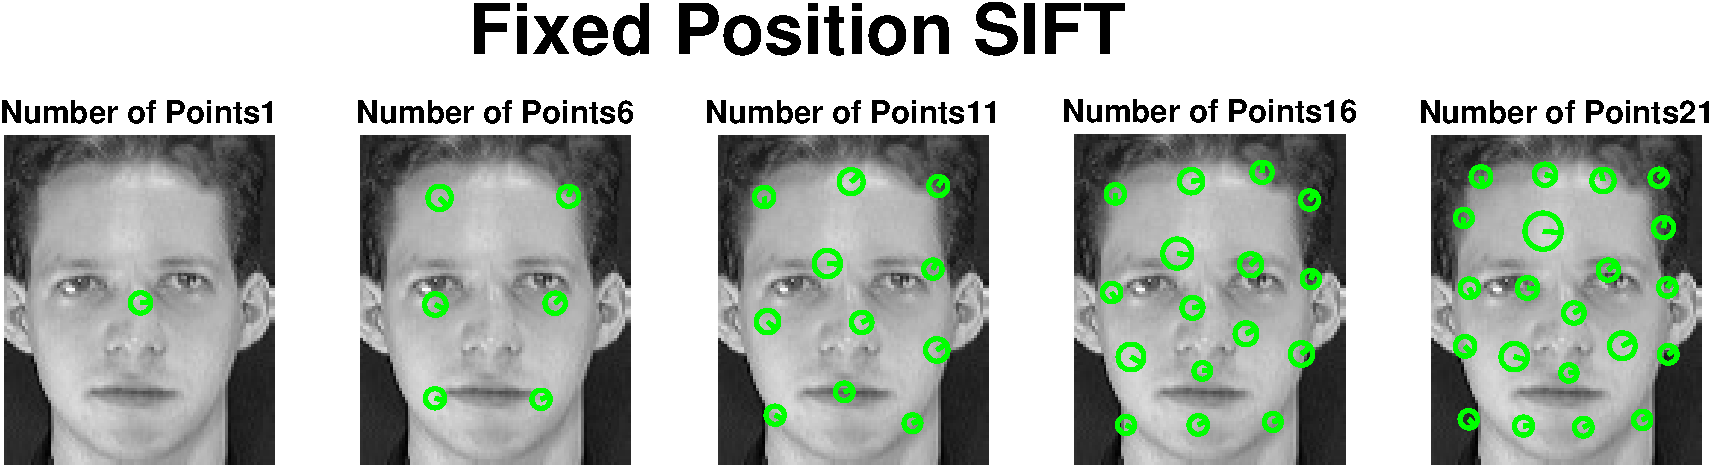
\includegraphics[width=\MyFactor\textwidth]{Img/c3/sift_fixedp} 
		\captionof{figure}{Kmeans计算出的特征位置}
		}
		\end{minipage}
		\medskip
		\end{center}
		
	第二步是在线在这些固定的特征点计算对应特征空间的描述,和之前方法的第4步一致.计算出的特征空间的描述的全集就可以作为输入图像的全局特征.


\subsection{NBNN分类法}
由于SIFT的特性,本项目在上一节固定编码的同时,也结合SIFT特性实现了NBNN(Naive-Baysian Nearest Neighbor)算法\cite{boiman2008defense}.NBNN算法不需要对SIFT进行特殊的编码,同时可以并行运算.它是基于距离的运算,主要思想是:
	\begin{enumerate}
		\item 通常的编码方法,如BoW丢失了很多有用的细节信息,只是注意到了描述空间中的高频成分,但是通常来说样本最具区分性的特征空间是其低频成分.并不适合以计算距离为主的KNN算法
		\item 通常的编码算法中,计算的是图像和图像之间的距离,这限制了算法的泛化能力.应该计算图像和类别之间的距离.
	\end{enumerate}
	它的主要过程是:
	\begin{enumerate}
		\item 对于样本图片,求得每类所有图片的所有描述
		\item 对于测试图片,求得该张图片的所有描述
		\item 在某个类别的所有描述的空间内,搜索测试图片的每个描述的最近特征点,并求得它们总共的距离.也即求得:
			\begin{equation}
				dis = \Sigma_{i=1}^n  || d_i - NN_C(d_i)^2||
			\end{equation}
			其中$NN_C(d_i)$是特征$d_i$在类别C内最近的特征点.
			
		\item 对所有的类别都求得该距离,距离最近的就是测试图片所属的类别.
	\end{enumerate}

其缺点是涉及了很多的求最近点的过程,在没有优化的Matlab代码中,使用了KD树结构也需要很多时间才能完成分类.这部分原因是因为Matlab是脚本语言,对处理多重循环的速度不够快导致的,但是,同样不可否认这其中确实存在了很多的寻最近点的KD树查询过程.

\paragraph{NKNN并行加速}
值得一提的是,由于NKNN算法过于缓慢,笔者使用了CPU并行运算.它具体的加速部分是加速了之前描述的步骤1和步骤3,步骤1是构架KD森林的过程,花费时间并不多.步骤3是遍历KD森林的过程,是程序主要耗时的地方.对于每个测试样本,它需要让这个样本逐一和ORL数据库中40个类构成的KD树逐一求得最小距离,使用了多核加速后,从以前的一次查询一个类加速到了一次查询两个类.\newline


无论如何,KBNN算法只是基于距离的计算,可以被并行加速,同时有很高的识别度.

\section{相关实验}
参见\ref{sec:comp_local}.
